%Author: Marius
\label{sec:fixed_data}
After working with our fake data streams for some time, we were provided with some real data by BMW. The data was presented in two different formats: Flowlogs and Metrics. They contained network traffic information  starting from December 21, 2018. 
Flowlogs contain raw information about network traffic, e.g. which IP-adress made a request to which server at which point along with other details.

In this section, we will focus on how we used the Metrics files. The Metrics already accumulate the raw network traffic information from the Flowlogs and only give us information about the amount of traffic. More specifically, they contain the amount of successful requests (with HTTP-Code 200) and failed requests (HTTP-Code 4xx and 5xx) at a certain time. Although the files were named \textit{output-mass.json}, they were not correctly encoded in JSON format. An example entry from one of the files can be seen in \ref{lst:metrics_example}.

\begin{minipage}{\linewidth}
\begin{lstlisting}[caption={Example entry from metrics data},label={lst:metrics_example}]
{
    [...]
    'response-code-4xx': {
    [...]
        'Datapoints': [
            {'Timestamp': datetime.datetime(2018, 12, 15, 11, 20, tzinfo=tzlocal()), 
            'SampleCount': 6.0, 
            'Unit': 'None'
            }
        ]
    }
}
\end{lstlisting}
\end{minipage}

Some efforts were made to parse the files with a python script. Once all the files are parsed, we take the \textit{SampleCount} values for each entry, and sort them into buckets according to their \textit{Timestamp}. For the time being, we did not differentiate between successful or failed requests, however, this might be a useful thing to do in the future. The buckets were chosen to be of 5 minute granularity in the final product, however we also experimented with 1 minute buckets.
\begin{figure}[h]
    \centering
    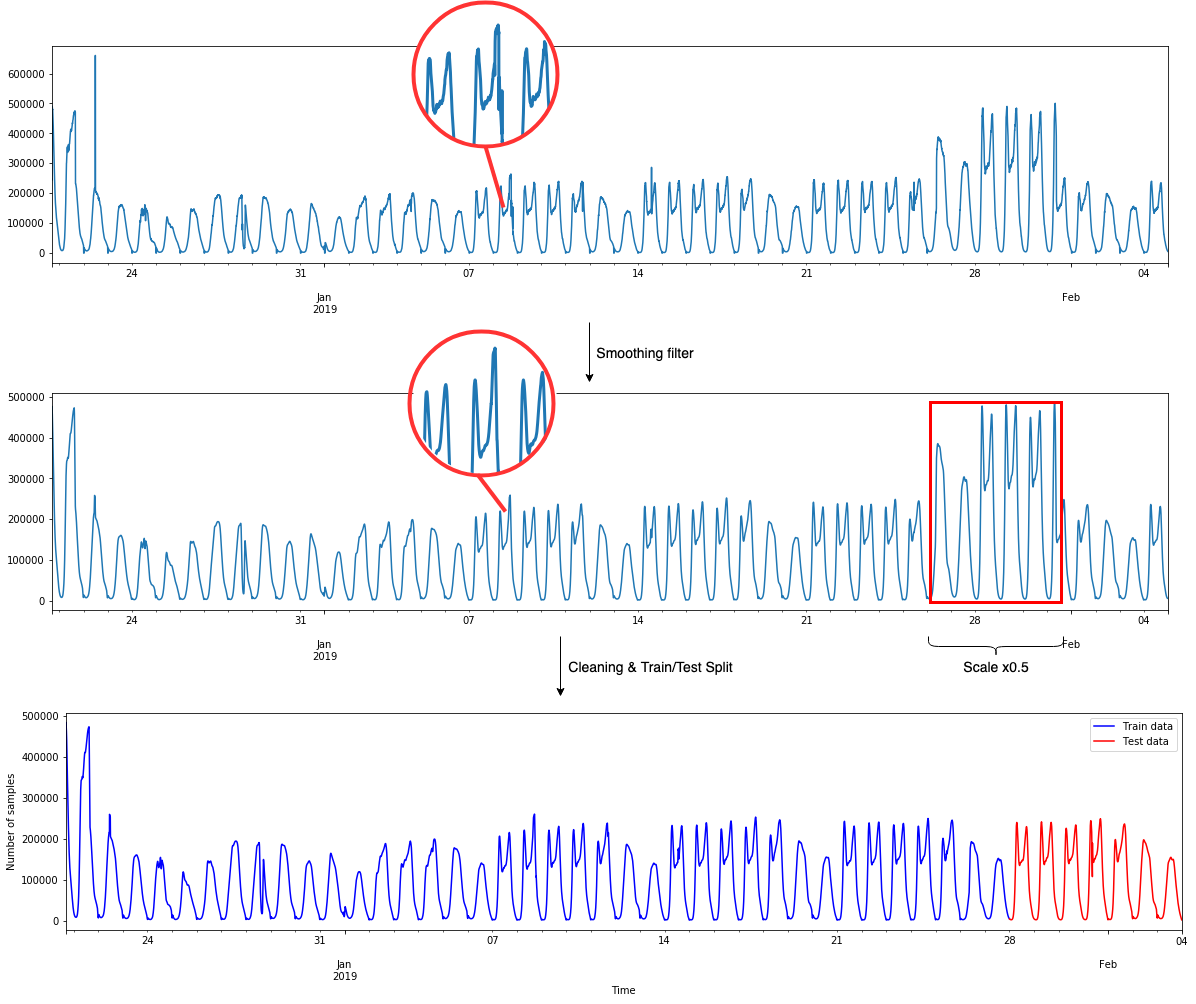
\includegraphics[width=1\textwidth]{images/data_preprocessing.png}
    \caption{Data preprocessing pipeline}
    \label{fig:data_preprocessing}
\end{figure}
\afterpage{\FloatBarrier}
A smaller bucket size means higher responsiveness in a real time anomaly detection model, since in order to react to incoming data, we have to wait until the current bucket is full. Furthermore, if the bucket size gets to small, the machine learning model might get vulnerable to noise. Larger buckets on the other side compress the training data for better usability and can make the model more robust. Next, we summed up the value in every bucket to obtain the raw time series, which can be seen in figure \ref{fig:data_preprocessing} in the first picture. 
\paragraph{Preprocessing and Cleaning} 
We noticed that the data is still very noisy and contains some impurities. For example, the data between the 26th and the 31st of January was scaled up by a factor of two for unknown reasons.
We reduced the noise by applying a smoothing convolution to the data, and scaled down the aforementioned interval (cf. fig. \ref{fig:data_preprocessing}).
One might argue that in timeseries data, the value of one point in time is highly correlated to the previous ones. Smoothing the timeseries exploits this property to get rid of sudden and unexpected jumps in the training data, or in other words, we reduce outliers and make training of our machine learning models more robust.
Finally, we separated one week of data for testing purposes.
\paragraph{Exporting for Machine Learning Models}
For further use with the Machine Learning models described later, the data had to exported in different formats. For the Random Cut Forest and the Mean Predictor, the data can be provided in a simple CSV Format with \textit{Timestamp} and \textit{Value}. The DeepAR Model however requires a more complex format which is described more deeply in chapter \pageref{ch:deepar}.
\paragraph{Advantages and Disadvantages}
While extracting the data from the metrics files is convenient and simple, this approach has several drawbacks: Although we do not have further insight about this, we suspect the metrics files are not generated in realtime, because they accumulate data observed in one day. Thus they can only be used for pretraining a model with fixed data. We have no control over how the metrics files are accumulated. In order to obtain full control over the data stream, one must work with the raw flowlogs files. An approach that utilizes the flowlogs data from scratch is described in section \ref{sec:real_time_anomaly_detection}

